% Beamer slide template prepared by Tom Clark <tom.clark@op.ac.nz>
% Otago Polytechnic
% Dec 2012

\documentclass[10pt]{beamer}
%\usetheme{Dunedin}
\usepackage{graphicx}
\usepackage{fancyvrb}
\usepackage{ulem}
\newcommand\codeHighlight[1]{\textcolor[rgb]{1,0,0}{\textbf{#1}}}

\title{Introduction to Nagios}
\author[IN719]{Systems Administration}
\institute[Otago Polytechnic]{
  Otago Polytechnic \\
  Dunedin, New Zealand \\
}
\date{}

\begin{document}

%----------- titlepage ----------------------------------------------%
\begin{frame}[plain]
  \titlepage
\end{frame}

%----------- slide --------------------------------------------------%
\begin{frame}
  \frametitle{Our Problem}
  
\begin{itemize}
\item We need to know when things break. 
\item We want to know about problems \emph{before} things break.
\end{itemize}
\end{frame}


%----------- slide --------------------------------------------------%
\begin{frame}
  \frametitle{Proposed Solutions}
  
\begin{itemize}
\item \sout{We perform various service checks on our systems regularly.} 
\item \sout{We write some scripts to automate these steps.}
\item \sout{???}
\item \sout{Profit!}
\item We use a centralised monitoring tool.
\end{itemize}
\end{frame}


%----------- slide --------------------------------------------------%
\begin{frame}
  \frametitle{Monitoring Tools}
  
\begin{itemize}
\item Nagios
\item Icinga
\item Zabbix
\item Spiceworks
\end{itemize}

Nagios is the best known and most widely used of these and is the one we will use in this paper.
\end{frame}


%----------- slide --------------------------------------------------%
\begin{frame}
  \frametitle{Example Scenario}
  
\begin{itemize}
\item We have a server, db.op-bit.nz, running the MySQL DBMS.
\item We want to monitor server uptime and the MySQL service.
\item One systems admin should be notified of any issues.
\item We will use puppet to manage the Nagios config.
\end{itemize}

\end{frame}

%----------- slide --------------------------------------------------%
\begin{frame}
  \frametitle{The Plan}
  
  We will define the following nagios resources in our Nagios Puppet module
\begin{itemize}
\item host:  db.op-bit.nz
\item hostgroup with our host as a member
\item contact and contactgroup for the admin
\item service:  MySQL
\end{itemize}
\end{frame}

\begin{frame}
\frametitle{Configuration File Overview}
\hspace{-2cm}
%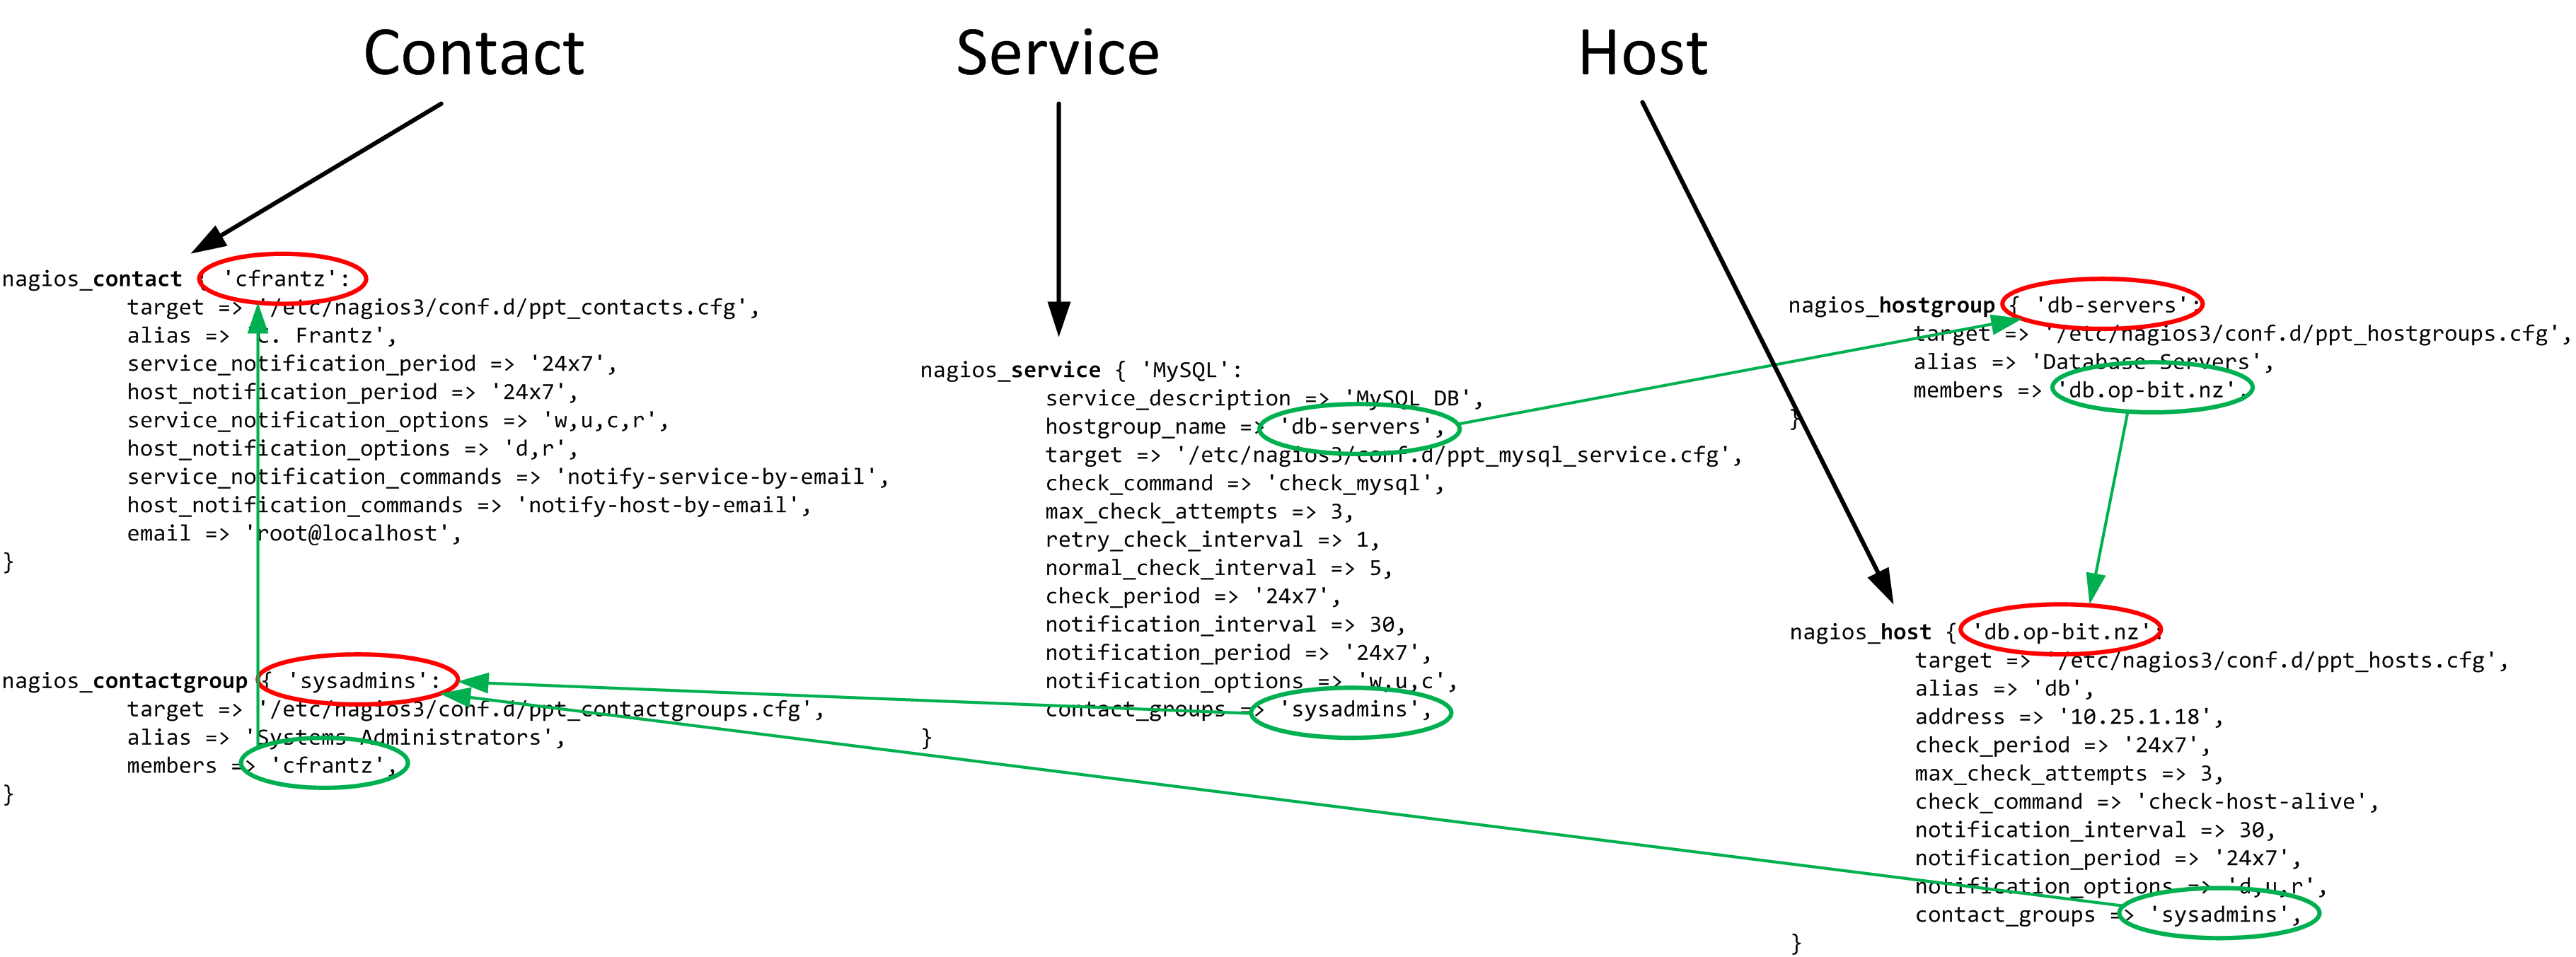
\includegraphics[width=1.2\textwidth]{Nagios_Configuration_Structure.png}

\vspace*{\fill}

% Your image goes here
\noindent
\makebox[\textwidth]{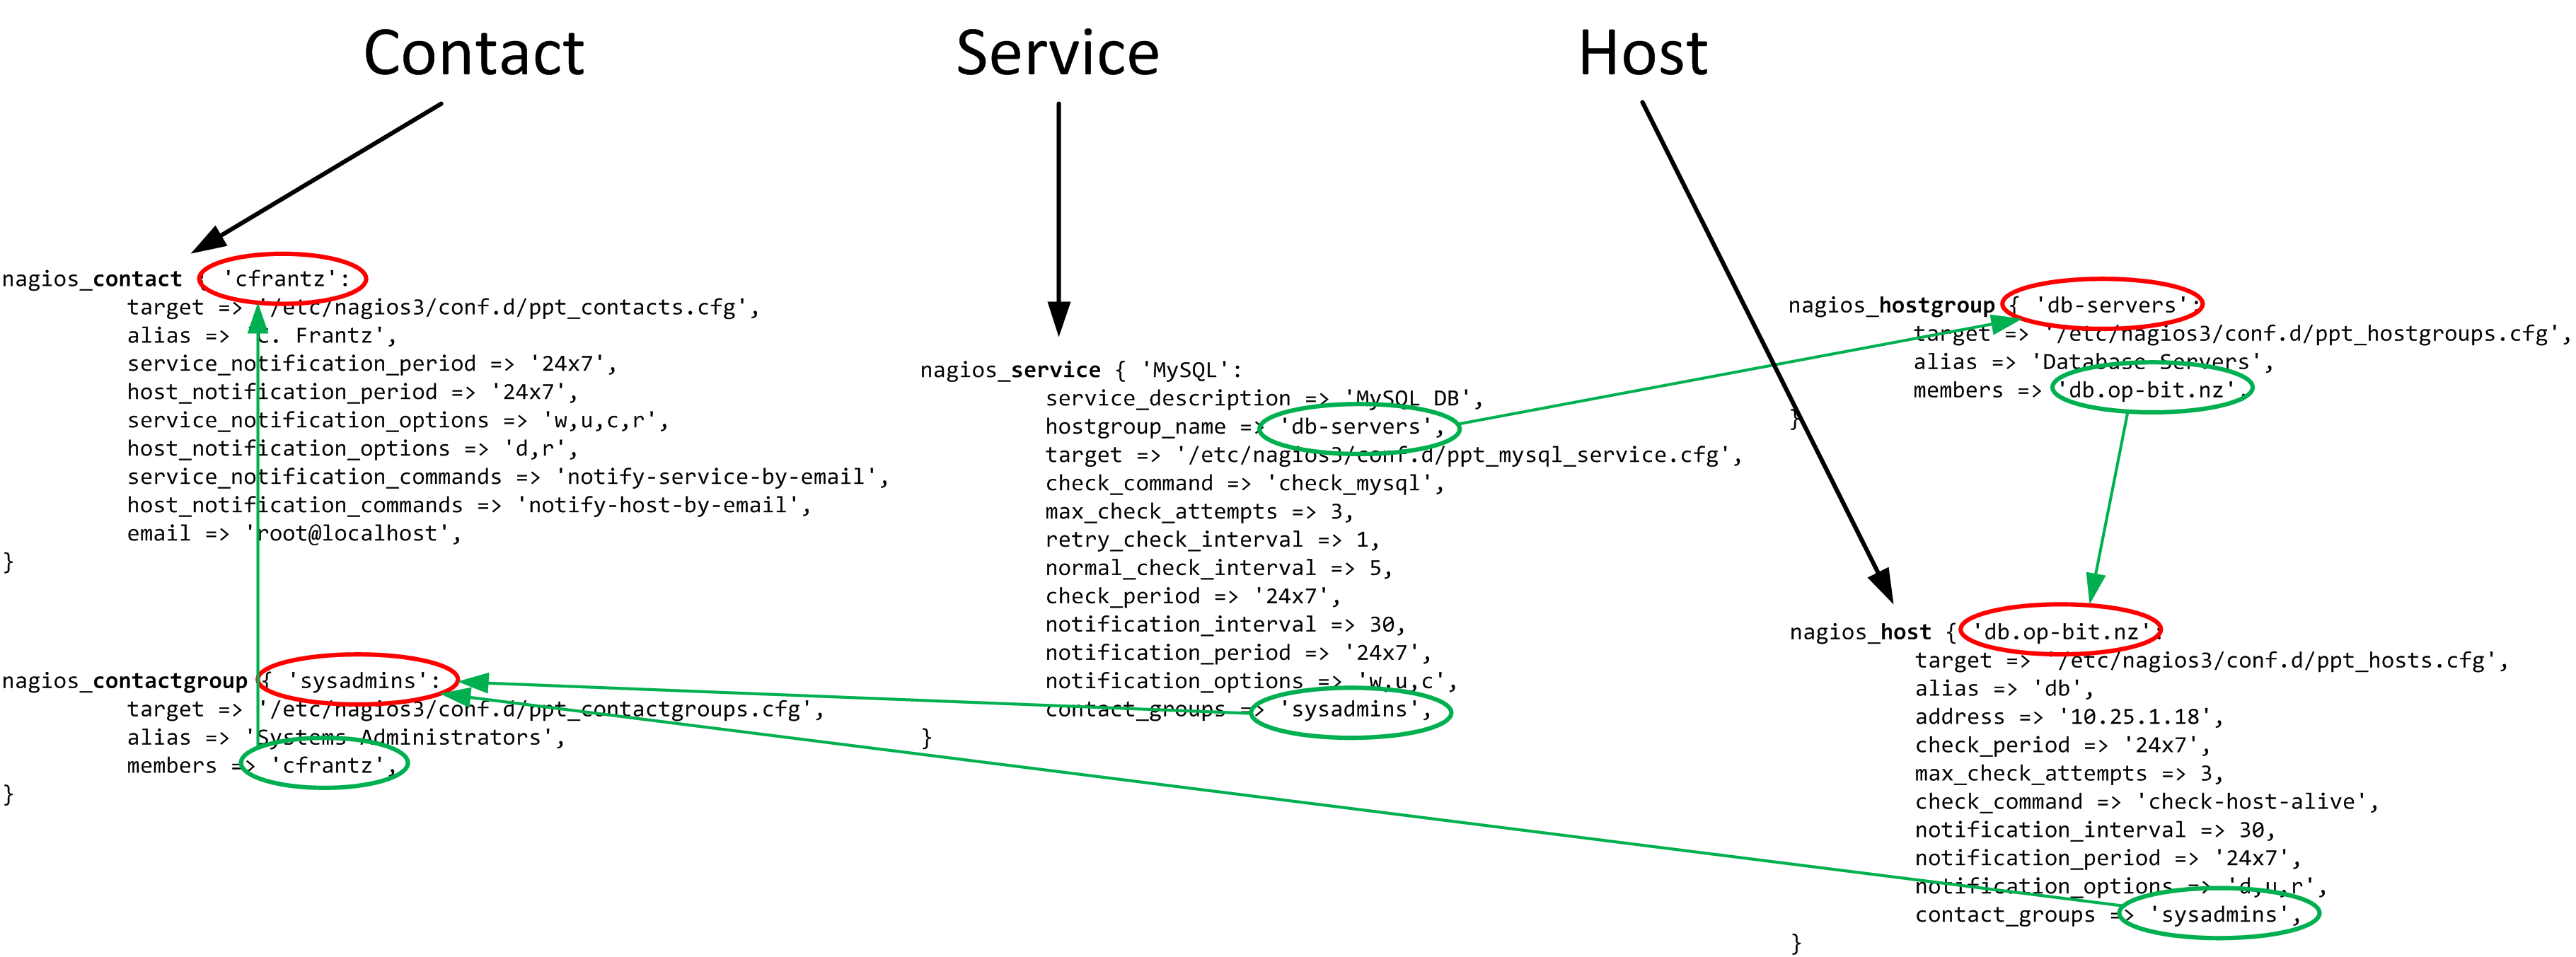
\includegraphics[width=1.15\textwidth]{Nagios_Configuration_Structure.png}}%

\vspace*{2cm}

\end{frame}



%----------- slide --------------------------------------------------%
%\begin{frame}[fragile]
  %\frametitle{Host}
%\begin{verbatim}
%%nagios_host { 'db.op-bit.nz':
                 %%target => '/etc/nagios3/conf.d/ppt_hosts.cfg',
                 %%alias => 'db',
                 %%address => '10.25.1.18',
                 %%check_period => '24x7',
                 %%max_check_attempts => 3,
                 %%check_command => 'check-host-alive',
                 %%notification_interval => 30,
                 %%notification_period => '24x7',
                 %%notification_options => 'd,u,r',
                 %%contact_groups => 'admins',
              %%}
%\end{verbatim}
 %\end{frame}
%----------- slide --------------------------------------------------%
%\begin{frame}[fragile]
  %\frametitle{Host Group}
  %\begin{verbatim}
%
  %nagios_hostgroup{'db-servers':
              %target => '/etc/nagios3/conf.d/ppt_hostgroups.cfg',
              %alias => 'Database Servers',
              %members => 'db.sqrawler.com',
  %}
%
	  %\end{verbatim}
 %\end{frame}
%%----------- slide --------------------------------------------------%
%\begin{frame}[fragile]
  %\frametitle{Contact}
  %\begin{verbatim}
  %nagios_contact { 'tclark':
              %target => '/etc/nagios3/conf.d/ppt_contacts.cfg',
              %alias => 'Tom Clark',
              %service_notification_period => '24x7',
              %host_notification_period => '24x7',
              %service_notification_options => 'w,u,c,r',
              %host_notification_options => 'd,r',
              %service_notification_commands => 'notify-service-by-email',
              %host_notification_commands => 'notify-host-by-email',
              %email => 'root@localhost',
  %}
	  %\end{verbatim}
 %\end{frame}
%%----------- slide --------------------------------------------------%
%\begin{frame}[fragile]
  %\frametitle{Contact Group}
  %\begin{verbatim}
  %nagios_contactgroup { 'sysadmins':
               %target => '/etc/nagios3/conf.d/ppt_contactgroups.cfg',
               %alias => 'Systems Administrators',
               %members => 'tclark',
  %}
	  %\end{verbatim}
 %\end{frame}
%%----------- slide --------------------------------------------------%
%\begin{frame}[fragile]
  %\frametitle{Service}
  %\begin{verbatim}
  %nagios_service {'MySQL':
              %service_description => 'MySQL DB',
              %hostgroup_name => 'db-servers',
              %target => '/etc/nagios3/conf.d/ppt_mysql_service.cfg',
              %check_command => 'check_mysql',
              %max_check_attempts => 3,
              %retry_check_interval => 1,
              %normal_check_interval => 5,
              %check_period => '24x7',
              %notification_interval => 30,
              %notification_period => '24x7',
              %notification_options => 'w,u,c',
              %contact_groups => 'sysadmins',
  %}
	  %\end{verbatim}
 %\end{frame}

\end{document}
